\begin{figure*}[htbp]
    \centering
    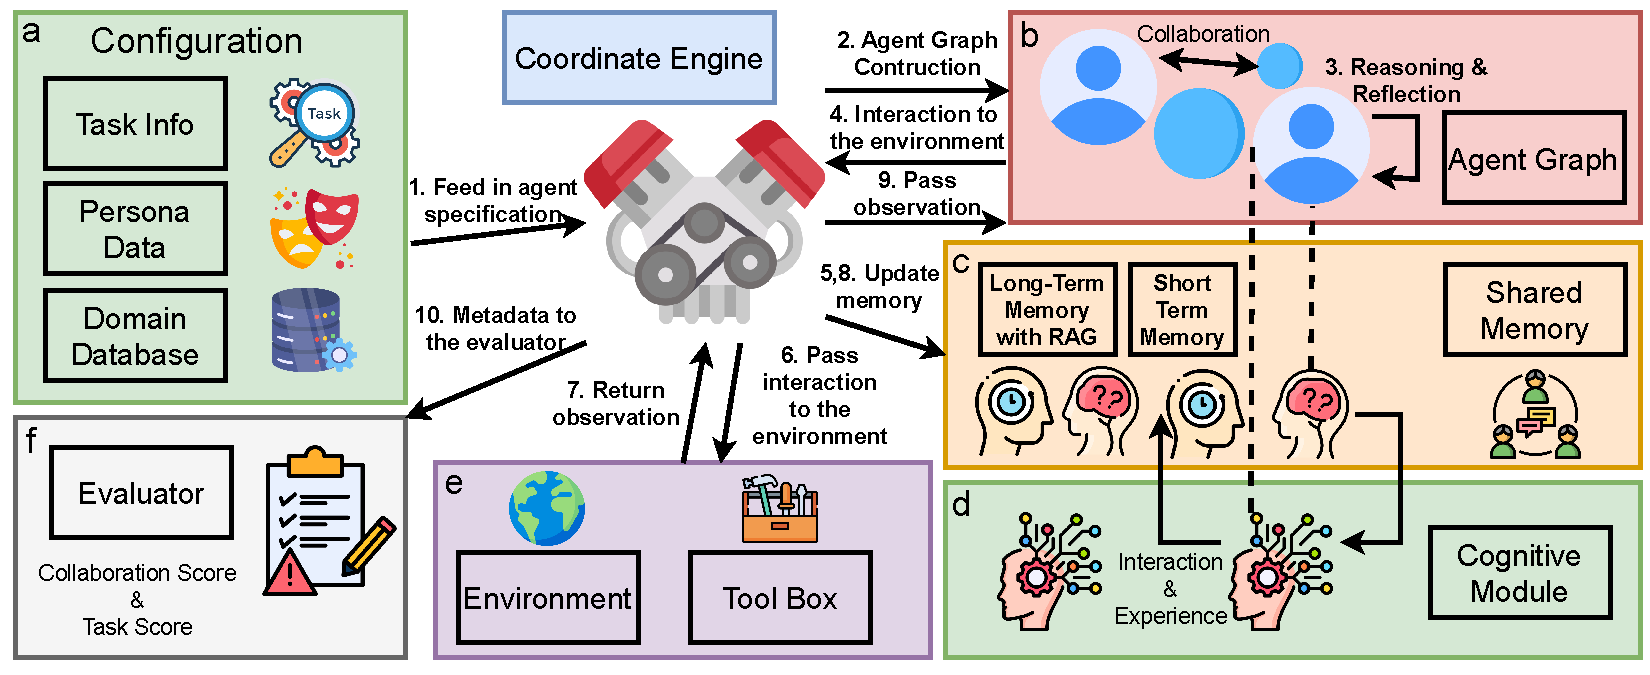
\includegraphics[width=\linewidth]{graphs/engine.pdf}
    \caption{MARBLE \icon: coordination engine과 cognitive module을 통해 과제 정보, persona data, domain database, memory module, 환경 사이의 상호작용을 보여 준다.}
    \label{fig:engine}
\end{figure*}

\section{관련 연구}
% Existing works on LLM-driven multi-agent systems, such as AgentBench~\citep{liu2024agentbench} and VisualAgentBench~\citep{liu2024visualagentbenchlargemultimodalmodels}, primarily focus on single-agent tasks. Recent studies have explored agent collaboration in various domains like scientific problem solving~\citep{tang2024prioritizing, chan2024mlebenchevaluatingmachinelearning}, coding~\citep{jimenez2024swebench}, and gaming~\citep{wang2023voyageropenendedembodiedagent}. However, a holistic evaluation framework that comprehensively analyzes coordination, role differentiation, and emergent agent behavior is still missing.

% We compare our framework with existing benchmarks and focus on expanding the evaluation to multi-agent settings, emphasizing the importance of planning, communication, and shared and individual memory capabilities in agent systems.

\subsection{LLM 기반 다중 에이전트 시스템}

LLM 기반 다중 에이전트 시스템은 여러 도메인에서 협업적 문제 해결을 가능하게 했다~\citep{Park2023GenerativeAgents, li2023camelcommunicativeagentsmind, chen2023agentversefacilitatingmultiagentcollaboration}. 이러한 시스템은 문헌 검토와 실험 설계를 통해 과학 연구를 지원하고 \citep{zhou2024hypothesis, agarwal2024litllmtoolkitscientificliterature}, 코드 생성과 유지보수 \citep{bouzenia2024repairagent}를 포함한 소프트웨어 공학 과제 \citep{huang2023agentcoder, wu2023autogen, zhou2023agents, hong2024metagpt, ishibashi2024self, islam2024mapcoder, openhands, zhugegptswarm}, 게임 응용 \citep{chen2023gamegpt}에도 활용된다. Minecraft에서는 에이전트가 건설부터 내비게이션까지 복잡한 과제를 수행한다 \citep{wang2023voyageropenendedembodiedagent, chen2023agentversefacilitatingmultiagentcollaboration, yu2024minelandsimulatinglargescalemultiagent, dong2024villageragentgraphbasedmultiagentframework}.

% In gaming, LLM-powered agents simulate human-like behavior and contribute to creating more realistic environments. For example, GameNGen, the first neural-driven game engine, enables real-time interaction in complex environments, simulating games like DOOM at over 20 frames per second on a single TPU \cite{valeveski2024diffusion}. Similarly, MindAgent introduces CUISINEWORLD, a novel gaming scenario and benchmark for evaluating multi-agent collaboration efficiency, enabling agents to collaboratively play games and solve tasks \cite{gong2023mindagent}.

% In world simulation scenarios, these multi-agent systems excel in tasks that require judgment, self-awareness, and strategic decision-making. For example, multi-agent LLM systems have been applied to games like \textit{Chameleon} and \textit{Undercover}, where they demonstrate abilities in social deduction and deception, as well as in game theory scenarios like \textit{Cost Sharing} and \textit{Public Goods}, which highlight their capacity for strategic collaboration and resource management. \citep{xu2023magic}
% Additionally, these systems are applied in healthcare for more accurate diagnostics and decision making\citep{ke2024enhancing, kim2024adaptive}. In the business world, multi-agent LLM systems optimize tasks such as customer support, sales, and operational workflows \citep{chen2024agentverse}. Moreover, in education, multi-agent systems are used for personalized tutoring and collaborative learning \citep{gosling2024multi}. LLM-based multi-agent systems are also utilized in urban planning, logistics, and resource management, enhancing decision-making through simulations and coordination \citep{zhou2024largelanguagemodelparticipatory}. Despite these successes, challenges remain, including ensuring effective communication among agents, handling emergent behaviors, and scaling these systems for real-world applications \citep{agashe2024llmcoordinationevaluatinganalyzingmultiagent}. These issues highlight the need for robust frameworks to assess and improve multi-agent coordination, which our work aims to address.
GameNGen은 DOOM에서 실시간 상호작용을 가능하게 하고 \citep{valeveski2024diffusion}, CUISINEWORLD는 다중 에이전트 협업을 벤치마크한다 \citep{gong2023mindagent}. 응용 범위는 사회적 추론 게임, game theory \citep{xu2023magic}, healthcare \citep{ke2024enhancing, kim2024adaptive}, business \citep{chen2024agentverse}, education \citep{gosling2024multi}, urban planning \citep{zhou2024largelanguagemodelparticipatory}까지 확장된다. 진전에도 불구하고 communication, emergent behavior, scalability에는 여전히 문제가 남아 있으며 \citep{agashe2024llmcoordinationevaluatinganalyzingmultiagent}, 이는 강건한 평가 프레임워크의 필요성을 뒷받침한다.

% \kunlun{More Comparison between the existing benchmarks make a table}
% \kunlun{adding more work like waragent,}

\subsection{다중 에이전트 협업}

% The success of single LLM-based agents in reasoning and planning has inspired collaborative frameworks involving multiple LLM agents, enabling the integration of specialized capabilities and often surpassing the performance of individual models \citep{zhang2023exploring}. Communication topologies explored for multi-agent collaboration include non-interactive setups where agents operate independently, chain structures where outputs are passed sequentially, star configurations with a central agent directing others, hierarchical tree arrangements with parent-child relationships, and complex graph-based systems facilitating dynamic interactions \citep{zhou2024hypothesis}. Recent studies have introduced dynamic communication strategies, enabling adaptive collaboration tailored to specific tasks. For instance, frameworks like G-Designer leverage graph neural networks to optimize multi-agent communication and coordination \citep{zhang2024gdesignerarchitectingmultiagentcommunication}. Despite these advances, evaluating aspects like coordination, role differentiation, and emergent behaviors in LLM-based systems remains challenging, emphasizing the need for a comprehensive evaluation framework, which our work seeks to address.

최근 다중 에이전트 시스템의 발전은 두 가지 상호보완적 scaling paradigm을 강조한다. 하나는 에이전트의 추론과 적응성을 강화하는 \textit{cognitive scaling}이고, 다른 하나는 대규모 에이전트 집단을 활용해 창발 행동을 이끌어내는 \textit{population scaling}이다 \citep{zhugegptswarm, qian2024scalinglargelanguagemodelbasedmultiagentcollaboration}.

Cognitive scaling은 dynamic architecture adaptation과 self-organizing coordination strategy 같은 메커니즘을 탐구하여 에이전트 의사소통의 가장 효과적인 패턴을 찾는다 \citep{zhugegptswarm}. 한편 population-based scaling은 에이전트 수가 증가하면서 hierarchy delegation, decentralized consensus 등 다양한 협업 패턴을 통해 집단적으로 상호작용할 때 비선형적 성능 향상을 보인다 \citep{qian2024scalinglargelanguagemodelbasedmultiagentcollaboration}.
이러한 접근은 지정학적 갈등 시뮬레이션 \citep{hua2024warpeacewaragentlarge}부터 과학적 발견 workflow \citep{zhou2024hypothesis, zhang2025crewfacilitatinghumanaiteaming}까지 복잡한 응용을 가능하게 한다.

% Recent advances in multi-agent systems reveal two complementary scaling paradigms: \textit{cognitive scaling} through dynamic architecture optimization \citep{zhugegptswarm} and \textit{population scaling} via agent orchestration \citep{qian2024scalinglargelanguagemodelbasedmultiagentcollaboration}. Cognitive approaches treat agents as optimizable computational graphs, achieving improved performance through automated topology pruning \citep{zhugegptswarm}, while population-based methods demonstrate logistic performance growth with agent count through irregular collaboration patterns \citep{qian2024scalinglargelanguagemodelbasedmultiagentcollaboration}. \heng{not sure what you mean by 'irregular collaboration patterns'. elaborate and illustrate?} \heng{'agent count through irregular collaboration patterns' very hard to parse} These paradigms enable complex applications ranging from geopolitical conflict simulation \citep{hua2024warpeacewaragentlarge} to scientific discovery workflows \citep{zhou2024hypothesis}.

% \kunlun{change the cognitive statement into something else, scaling in numbers, coordination strategies, emergent behaviors analysis, social, no taxonomy needed}

% Architectural innovations address core coordination challenges: Graph neural networks optimize communication efficiency \citep{zhang2024gdesignerarchitectingmultiagentcommunication}, while hierarchical structures enhance task decomposition \citep{zhou2024hypothesis}. Our benchmark extends these foundations through two axes: 1) \textit{Topology Robustness} testing across communication graphs, 2) \textit{Emergent Strategy Analysis} quantifying competitive adaptation. This framework reveals that automated topology optimization reduces coordination overhead by ??\% compared to fixed architectures \citep{zhugegptswarm}, while irregular collaboration patterns outperform regular structures in large-scale coordination \citep{qian2024scalinglargelanguagemodelbasedmultiagentcollaboration}.
% \kunlun{todo:make sure the data and content cited is accurate}


% \section{System Architecture and Design}
% The proposed multi-agent system architecture includes the following components:

% \subsection{Coordination and Task Completion}
% Figure~???????????????????????????????????????????????????????????????????????????????????????????????????????????????????????????????????????????????????????????????????????????????????????????????????????????????????????????????????????????????????????????????????????????\ref{fig:results} provides insights into the performance of agents across different task scenarios, and we find significant trade-offs between planning efficiency and task completion success.



% \begin{itemize}
%     \item \textbf{Coordination Engine}: Manages agent behavior, interactions, and constructs the agent graph for collaboration. Different collaboration strategies, such as group chatting and hierarchical planning, are implemented.
%     \item \textbf{Agent Graph}: Represents relationships among agents, enabling reasoning, reflection, and adaptive collaboration.
%     \item \textbf{Shared and Individual Memory}: Allows agents to retain both collective and individual knowledge, facilitating coordinated decision-making.
%     \item \textbf{Cognitive Module}: Supports adaptive behavior and evolving strategies with accumulated experience.
%     \item \textbf{Interactive Environment and Tool Box}: Provides agents with tools to interact with the environment and complete assigned tasks.
%     \item \textbf{Evaluator}: Measures agent performance across various dimensions, providing feedback to improve collaboration.
% \end{itemize}

% The information flow in our system starts with the coordination engine, which constructs an agent graph based on task data. The agents interact with the environment through the provided tools, while shared memory aids in collaboration. Figure~??????????????????????????????????????????????????????????????????????????????????????????????????????\ref{fig:progress} illustrates the architecture.




% \subsection*{Methodology}

% \begin{figure*}[t]
%     \centering
%     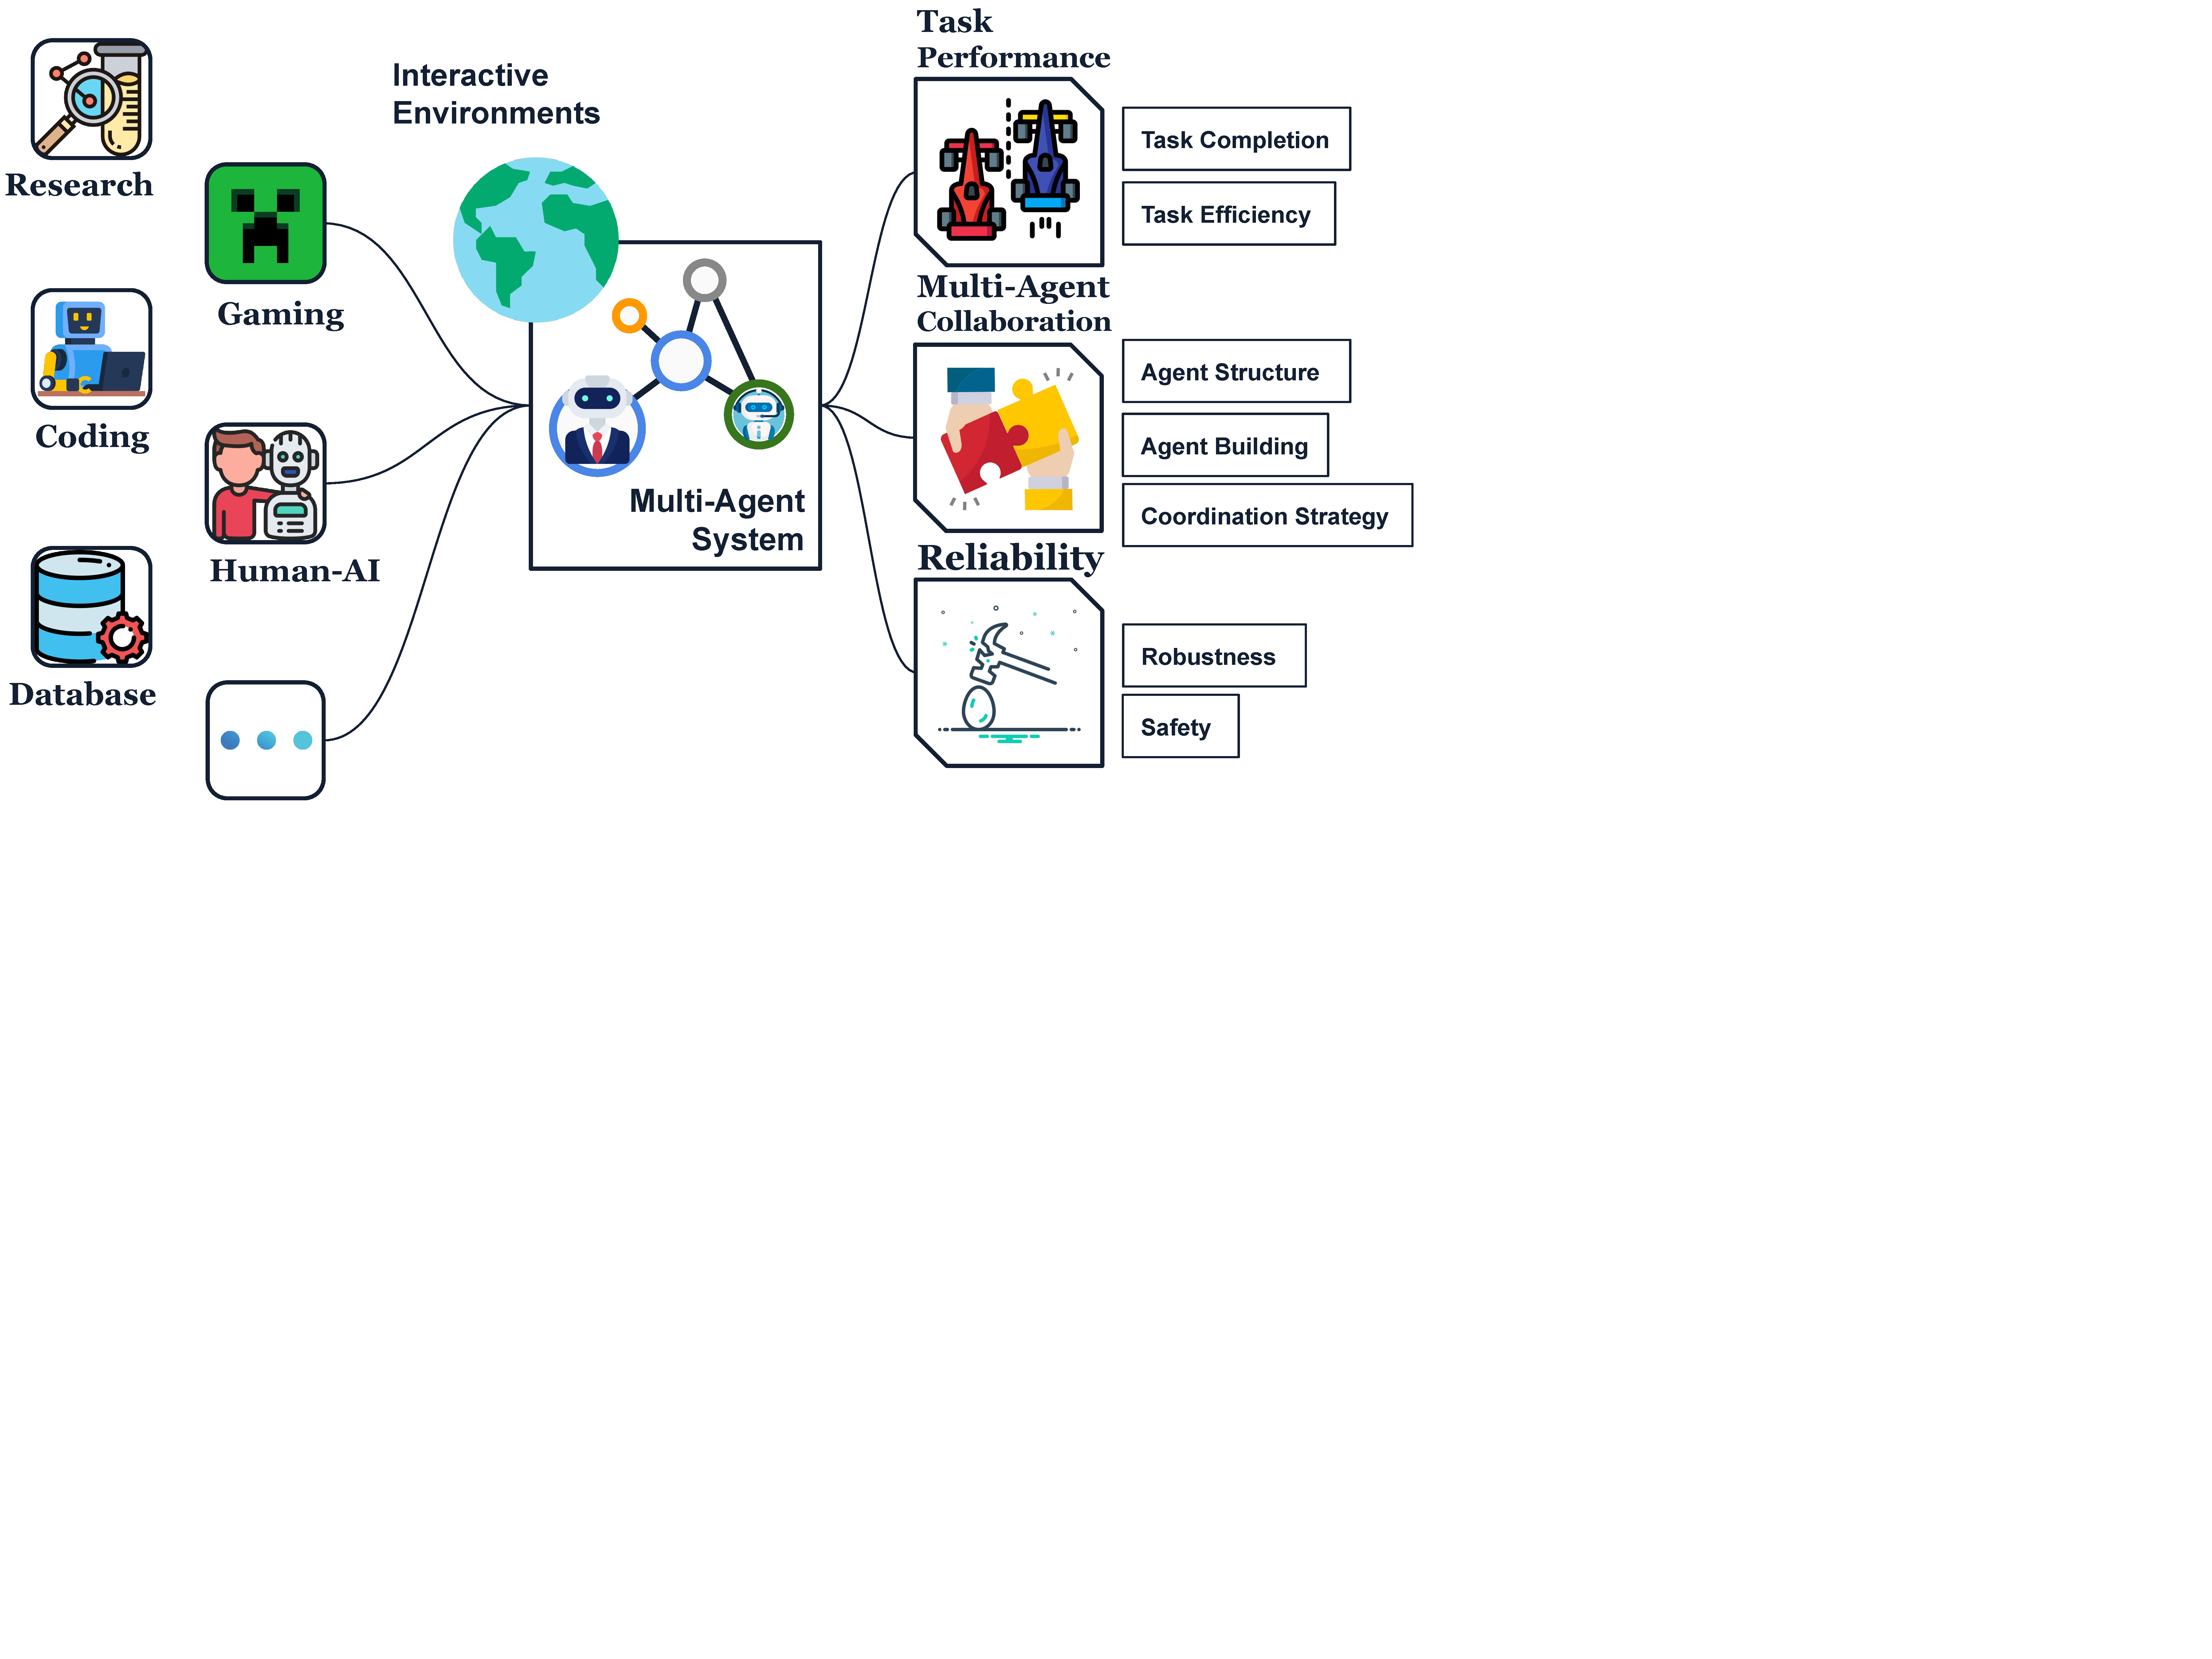
\includegraphics[width=0.96\linewidth]{graphs/Illustration.pdf}
%     \caption{The Main Multi-agent Eval Pipeline}
%     \label{fig:progress}
% \end{figure*}


% We designed a series of interactive environments for evaluating the multi-agent system. Each environment provides unique challenges, allowing us to assess aspects of task performance, collaboration, and reliability.

% The evaluation of the multi-agent system will be conducted through three major dimensions:

% \begin{itemize}
%     \item \textbf{Task Performance}: This dimension will focus on evaluating how effectively the agents complete assigned tasks. It will include metrics such as task completion and efficiency, providing insight into how well the agents achieve their objectives.
%     \item \textbf{Multi-Agent Collaboration}: In this dimension, we will assess the quality of collaboration among agents. We will evaluate aspects such as coordination strategies and workflow building to solve complex problems effectively.
%     \item \textbf{Reliability}: Reliability will be measured by analyzing the robustness and safety of the multi-agent system, ensuring stability under various conditions.
% \end{itemize}

% The system architecture consists of several interlinked modules:

% \begin{itemize}
%     \item \textbf{Coordinate Engine}: The coordinate engine orchestrates agent behavior by managing interactions and constructing the agent graph. The coordinate engine will include different collaboration strategy such as group chatting, hierarchical traverse planning, etc.
%     \item \textbf{Agent Graph}: The agent graph represents relationships among agents, enabling reasoning, reflection, and collaboration.
%     \item \textbf{Shared and Individual Memory}: Agents share a common memory for collective knowledge and maintain individual memory for personalized learning.
%     \item \textbf{Cognitive Module}: The cognitive module supports adaptive behavior, allowing agents to evolve with experience.
%     \item \textbf{Environment and Tool Box}: Agents operate within an interactive environment, using tools provided by the tool box to complete tasks.
%     \item \textbf{Evaluator}: The evaluator analyzes performance and provides feedback for improvement.
% \end{itemize}

% The flow of information starts with the coordinate engine constructing the agent graph based on task data. Agents interact with the environment using various tools, with shared memory facilitating collaboration.

% \textbf{Environment Module }: \zhaochen{todo below in the methodology part}

% \textbf{Memory Module} \xiaocheng{todo below in the methodology part}

% \textbf{Reasoning module}: \zhewang{todo below in the methodology part}

% \textbf{Milestone Generation Part}: \hongyi{To do in the benchmark part}
